
\chapter{Priprema podataka} % Main chapter title

\label{Priprema_podataka} % For referencing 

\section{Objedinjavanje CAFA3 i novijih \swissprot proteina}
\label{objedinjavanje}

Povezivanje CAFA3 proteina sa \swissprot unosima je jedini način da se dođe do
anotacija ključnim rečima. Takođe, dobijamo najnovije anotacije GO termina ali
i dodatne informacije, na primer taksonomsko poreklo proteina koje pomaže
razumevanju skupa podataka.

Iz CAFA3 trening skupa izdvojeni su svi validni proteini ( dužine barem 9 i
azbuke od 20 standardnih aminokiselina). U ovom koraku ne izbacujemo proteine
kraće od 40 AK.  Informacije o \swissprot bazi podataka dobijene su iz verzije
2017\_12, iz datoteke \file{uniprot\_sprot-only2017\_12.tar.gz} \cite{sprot}.
Navedena verzija sadrži 556 196 proteina.  Od 66 599 validnih CAFA3 proteina 66
530 ima nepromenjen \keyword{primarni identifikator}, ali 69 slogova u
\swissprot bazi sadrže nedostajuće CAFA3 identifikatore kao sekundarne. Kao što
je navedeno u Potpoglavlju \ref{svis-prot} ovo je posledica dva moguća
mehanizma:

\begin{enumerate}
  \item Unifikacija nekoliko CAFA3 proteina pod novi slog.
    Rezultat unifikacije prikazan je na Slici \ref{fig:unifikacija_slogova}. Analizom
    ovih promena uspešno su rekonstruisana svega četiri nova \swissprot sloga
    koja odgovaraju nedostajućim CAFA3 proteinima. Kako je četiri
    suviše mali broj, zbog jednostavnosti nismo ih ubrajali u dalju analizu
    te koristimo samo 66 530 slogova čiji primarni identifikatori su nepromenjeni.

  \begin{figure}[th]
  \centering
  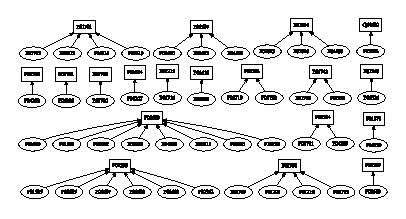
\includegraphics[scale=2]{plots/unifikacija_slogova2.eps}
  \decoRule
  \caption{Unifikacija starih(elipse) na nove slogove u \swissprot bazi podataka}
  \label{fig:unifikacija_slogova}
  \end{figure}

  \item Specijalizacija jednog CAFA3 proteina u više različitih slogova.  Zbog moguće
    statističke redundantnosti ovi slogovi su zanemareni.
\end{enumerate}


Validini CAFA3 proteini anotirani su sa  5 957 različitih GO termina Molekulske
Funkcije (MF) od kojih je 50 zastarelo i izbačeno iz \file{go.obo} datoteke.  U
\swissprot bazi podataka nismo bili u mogućnosti da proverimo samo za MF, ali
ukupno
je izbačeno 319 GO termina.
CAFA3 sadrži 67 MF koje se ne javljaju u \swissprot anotacijama dok \swissprot
sadrži 888 MF koje se ne javljaju u CAFA3 anotacijama.  Pošto je korišćena
verzija \swissprot baze novijeg datuma od CAFA3 podskupa, CAFA3 verzija
anotacija je zanemarena u korist novijih \swissprot anotacija. Ove informacije
sumirane su  Tabelom \ref{tab:godiff}

\begin{table}[htpb]
\begin{tabular}{|r|c|c|}
  \hline
                  & CAFA3 & \swissprot       \\
  \hline
  MF termini      & 5 957 &    7 471    \\
  nedostaje u go.obo   & 60 MF & 319 MF, CC i BP \\
  MF, samo u   & 67    & 888             \\
  \hline
\end{tabular}
  \centering
  \caption{Razlike u GO terminima između CAFA3 i \swissprot}
  \label{tab:godiff}
\end{table}

Dodatno, \swissprot sadrži 194 proteina čije se sekvence razlikuje u
odnosu na CAFA3 verziju proteina. Odlučili smo da zadržimo originalne CAFA3
sekvence.

\section{Grupisanje proteina po GO terminima}
\label{grupisanje}

Kao što je bilo reči u Sekciji \ref{ocenjivanje} sa $S_A$ označavamo skup
proteina koji obavljaju funkciju $A$, odnosno funkcija $A$ anotira proteine
grupisane skupom $S_A$.
Ako je GO termin $A$ potomak GO termina $B$ tj. važi $A$ \textit{is\_a} $B$ i
želimo da diskutujemo o funkciji $B$, onda i svi proteini koji imaju funkciju
$A$ (i time pripadaju skupu $S_A$) treba da budu sadržani i u skupu $S_B$.
Primetili smo da anotacije ključnih reči već podrazumevaju predloženo grupisanje.
Na primer, ključna reč \textit{Ribosomalprotein} anotira 1420 proteina, a
njen predak (uopštenje) \textit{Ribonucleoprotein} takodje anotira pomenutih 1420 proteina.
Anotacije GO terminima ne podrazumevaju ovako grupisanje već anotacije što
preciznije odgovaraju funkciji proteina. 
 
Za implementaciju predloženog grupisanje koristili smo algoritam topološkog
sortiranja. Ovako formirani skupovi koji sadrže manje od 20 proteina nisu bili
od značaja za dalju analize zbog čega su odbačeni.
Ovom metodom dobijeno je 1781\footnote{Bez ovog grupisanja imali bi samo 1146
MF termina  koji zadovoljavaju limit od min.  20 proteina} MF termin (od ukupno
11 135 validnih MF termina) sa minimum 20 pridruženih proteina uključujući i
koreni\footnote{koreni termin ili koreni čvor ontologije tj.  termin molekulska
funkcija} termin. U ovom koraku uračunati su samo proteini minimalne dužine 40
AK.

% \section{Ontologije gena i ključne reči}
\section{Mapiranje između GO termina i \swissprot ključnih reči}
\label{kw2go_mapiranje}

Kako je ovo istraživanje ograničeno na molekulske funkcije, u daljem tekstu biće
razmatrana mapiranja isključivo između ključnih reči kategorije MF koje zovemo
\keyword{MF ključne reči} i GO termina imenskog prostora MF koje zovemo
\keyword{MF termini}. Pokazaćemo da ovo nije trivijalan zadatak i da u opštem
slučaju zbog razlika u nomenkulaturi mapiranje ne postoji ili nije ekvivalentno
originalnoj funkciji.

U originalnom radu navodi se da je \swissprot baza sadržala 143 MF ključne
reči.  Datoteka \file{keywlist.txt} \cite{keywlist_txt} iz 20.12.2017 sadrži
195 MF ključnih reči.  Nažalost, nismo pronašli originalnu \file{keywlist.txt}
datoteku pa  ne znamo egzaktnu razliku, ali jasno je da su neke ključne reči
izbačene ili zamenjene a neke samo dodate. Datoteka \file{keywlist.txt} opisuje
ključne reči, a sadrži i pridruživanja (relaciju) odgovarajućim GO terminima.
Pomenuta relacija pridružuje MF ključne reči ne samo MF terminima već i BP i CC
terminima. Strogo posmatrano pridruživanja ne čine funkciju (mapiranje), jer se
neke ključne reči preslikavaju u nekoliko GO termina čak i ako ograničimo sliku
preslikavanja na samo MF\footnote{Samo \textit{DNA invertase} se preslikava u
dva različita MF termina (\textit{DNA binding} i \textit{recombinase
activity})} ili samo BP termine.  Ipak, opisana
pridruživanja nazivaćemo mapiranja ili direktna mapiranja. Direktna mapiranja
za MF ključne reči opisana su Tabelom \ref{tab:direktna_map}.  Za 20 ključnih reči
uopšte ne postoji mapiranje dok je broj mapiranja ka MF, BP i CC terminima,
redom 104, 54 i 11. Dakle, veliki broj mapiranja ka MF terminima nedostaje.

\begin{table}[htpb]
\begin{tabular}{|r|c|c|c|c|c|}
  \hline
                   & ukupno & nema map. &  MF map. & BP map. & CC map.      \\
  \hline
   MF ključne reči & 195    &  20       &  104     & 54      & 11           \\
  \hline
\end{tabular}
  \centering
  \caption{Direktna mapiranja za MF ključne reči}
  \label{tab:direktna_map}
\end{table}

Nedostajuća direktna MF mapiranja pogotovo dolaze do izražaja za neuređene
klju- čne reči.  Slika \ref{fig:KWtop20dis} prikazuje direktna mapiranja za 20
najznačajnijih neuređenih MF ključnih reči preuzetih iz originalnog rada
\parencite{Xie2007}.  Tri ključne reči nemaju direktno mapiranje, dve se
mapiraju na ćelijske komponente, osam na biološke procese i svega šest na
molekulske funkcije dok ključna reč \textit{Antigen} više ne postojii. Sa druge
strane, od 20 uređenih MF ključnih reči samo jednoj fali direktno mapiranje.

\begin{figure}[!th]
\hspace*{-2.2cm} 
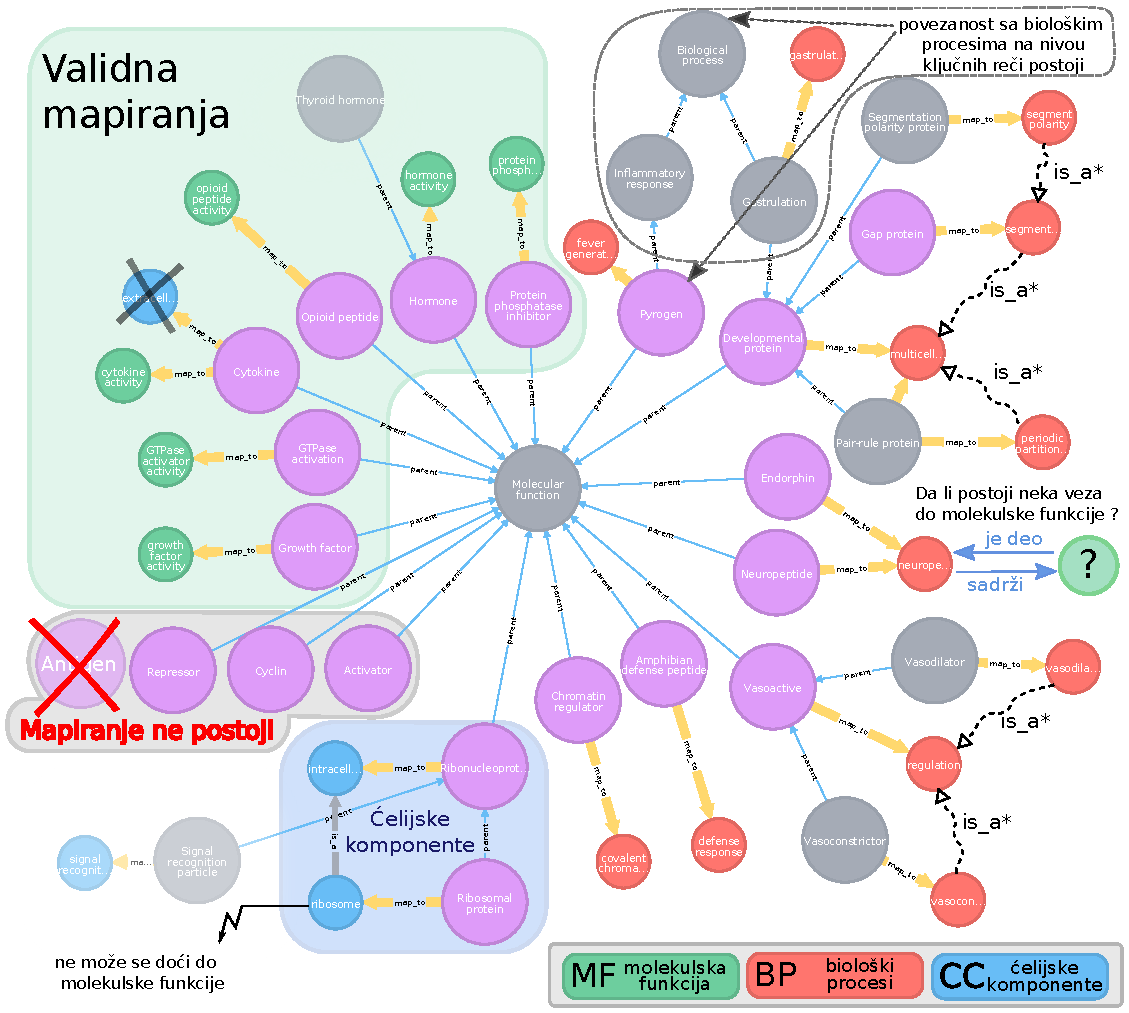
\includegraphics[scale=1]{Figures/plots/kw_dis2go.pdf}
\decoRule
\caption {
  Direktno mapiranje 20 najznačajnijih neuređenih MF ključnih reči \parencite{Xie2007}
  na GO termine.  Statistički značajne ključne reči su ljubičaste dok radi
  kompletnosti navodimo neke njihove specijalizacije i generalizacije koje su
  obojene sivo. GO termini su predstavljeni manjim kružićima.
}
\label{fig:KWtop20dis}
\end{figure}

Nedostajuća MF mapiranja (skoro polovina MF ključnih reči) ne samo da otežavaju
poređenje pojedinačnih ključnih reči već predstavljaju metodološki problem za
poređenje nomenkulatura.  Originalni rezultati su sortirani prema statističkoj
značajnosti (Z-skor za $F_j$) i predstavljaju dve tabele od 20 statistički
najznačajnijih neuređenih odnosno 20 uređenih MF ključnih reči zanemarujući
roditeljski odnos između njih. Na nivou ključnih reči ovo nije problem, ali ako
bi se isti postupak primenio na MF termine poredili bi manje od 200 ključnih
reči sa potencijalno preko 11 000 MF termina. Potrebno je odabrati dovoljno
opšte MF termine, takve da čine reprezentativan uzorak molekulskih funkcija i
da njihovo sortiranje po Z-skoru (kao u originalnom radu) ima smisla.  Biće
predložena dva pristupa za automatsko biranje opisanih MF termina dok je ručni
odabir izvan obima ovoga rada.  Oba pristupa imaju sličnu ideju, izdvojiti samo
one MF termine koji su pridruženi MF ključnim rečima. Međutim, kako polovina MF
mapiranja nedostaje (Tabela \ref{tab:direktna_map}), neophodno je dopuniti
nedostajuća mapiranja zarad smislenosti poređenja.  Automatski metodi koje ćemo
predložiti razlikuju se u načinu pronalaženja ovih nedostajućih mapiranja.
Treba primetiti da, čak i da nema nedostajućih mapiranja, ovaj pristup
zanemaruje statistički značajne MF termine koji nemaju ekvivalentne MF ključne
reči. 



\clearpage

\subsection{Metod indirektnih mapiranja}

Rezonujući nad relacijama ontologije gena, moguće je doći do
\keyword{indirektnih mapiranja} koja preko BP ili CC termina vode ka MF
terminima. Relacije \keyword{part\_of} i \keyword{has\_part} povezuju BP ili CC
sa MF terminima, ipak ove veze ne postoje uvek.  Traženje indirektnih mapiranja
izvršeno je korišćenjem \keyword{Neo4j} grafovkse baze. Za sve
ljubičaste BP termine sa Slike \ref{fig:KWtop20dis} i sve njihove
specijalizacije provereno je da li su nekom (bilo kojom) relacijom u vezi sa
nekim (bilo kojim) MF terminom. Pronađena je samo jedno indirektno mapiranje,
zajedničko za MF ključne reči \textit{Neuropeptide} i \textit{Endorphin}. Za tri
pomenuta CC termina indirektna mapiranja nisu pronađena. 


Razmotrimo pronađeno mapiranje za MF ključnu reč \textit{Neuropeptide} i
proteine koji su anotirani razmatranim funkcijama. Slika \ref{fig:neuropeptide}
generisana je \keyword{Cypher}\footnote{\textit{Cypher} je upitni jezik za
Neo4j grafovsku bazu} upitom koji koji pored GO termina takođe vraća anotirane
proteine. Preciznije, upit prvo pronalazi direktno mapirnje (BP termin)  a
zatim sve potomke (indirektne MF termine) i na kraju anotirane proteine.
Proteini su preuzeti iz CAFA3 skupa. 

{ \small
\begin{verbatim}
MATCH p=(:Keyword {name:"Neuropeptide"})--(:GOTerm)<-[*0..]-(:GOTerm)<--(:Prot)
RETURN p
\end{verbatim}
}

\begin{figure}[!th]
\centering
\hspace*{-1.0cm} 
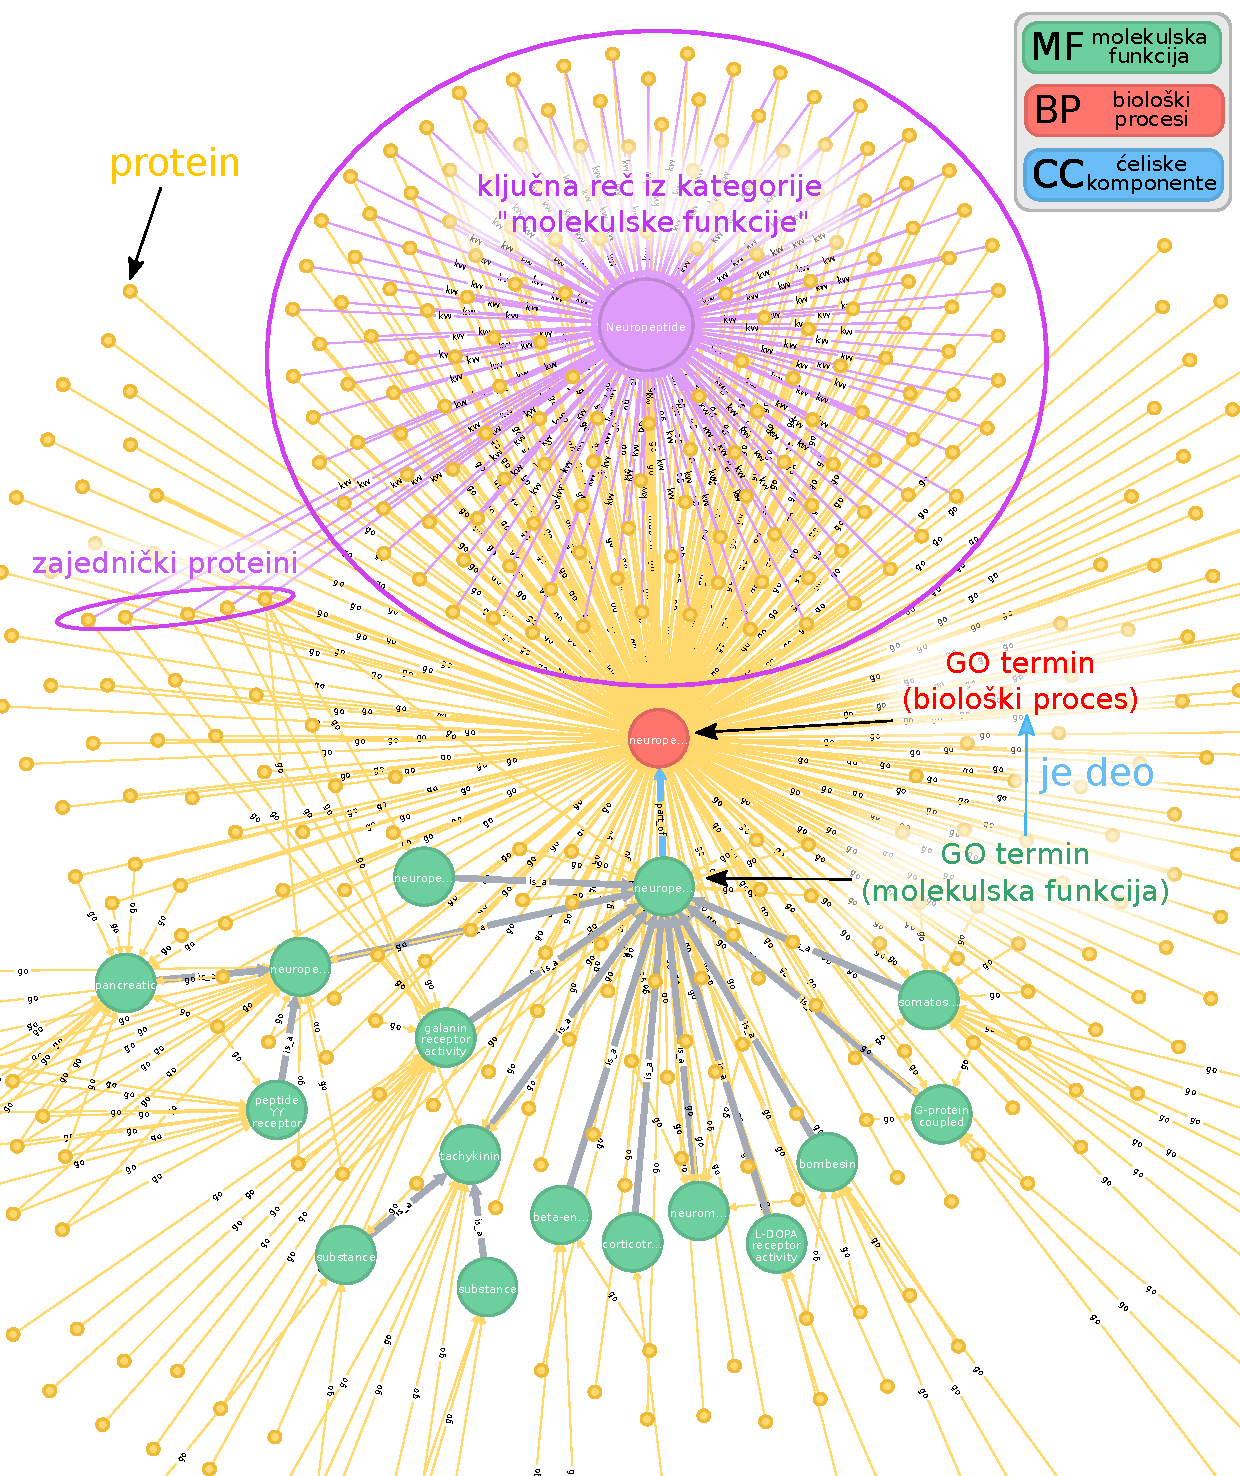
\includegraphics[scale=0.8]{Figures/plots/Neuropeptide2go.pdf}
\decoRule
\caption {
  Mapiranje ključne reči \keyword{Neuropeptide} na MF termin
  \textit{Neuropeptide receptor activity} preko relacije \keyword{part\_of}.
  Dobijeno mapiranje rezultuje malim brojem zajednički anotiranih proteina.
}
\label{fig:neuropeptide}
\end{figure}

Sa Slike \ref{fig:neuropeptide} jasno se uočava da ključna reč
\textit{Neuropeptide} deli svega 5 anotacija sa svim prikazanim MF terminima.
Smatramo da je zbog male sličnosti u anotacijama pronađeno indirektno
mapiranje nevalidno, jer se očigledno MF ključna reč \textit{Neuropeptide} i
MF termin \textit{Neuropeptide receptor activity} koriste u različitim
kontekstima. Zapravo, šablonski naziv pronađenog MF termina (po pravilima iz
Potpoglavlja \ref{MF}) označava da se termin koristi za anotiranje proteina
koji se \textit{vezuju za neuropeptid zarad inicijacije neke ćelijske
funkcije}, a ne samih neuropeptida. Takođe, treba primetiti da je pronađeni MF
termina povezan na BP termin relacijom \keyword{part\_of}.  Ovo može da
predstavlja još jedan razlog zašto je pronađeno mapiranje nevalidno.  Veza
\keyword{part\_of} podrazumeva agregaciju a ne kompoziciju. Agregacija
podrazumeva da  molekulska funkcija postoji nezavisno od biološkog procesa što
je suprotno od kompozicije koja predstavlja relaciju \keyword{has}. Nažalost,
nijedan od osam pomenutih BP termina nema relaciju \keyword{has} ka nekom MF
terminu.

\clearpage

Kao što je bilo reči u Potpoglavlju \ref{MF}, molekulske funkcije ne mogu da
predstavljaju gene ili genske produkte već funkcije koje oni obavljaju. Ključna
reč \keyword{Neuropeptide} po definiciji predstavlja peptide koje neuronske
ćelije oslobađaju ili hormone koji se oslobađaju iz drugih tipova ćelije. Jasno
je da ekvivalentan MF termin ne može da postoji.  Nažalost, postoji veliki broj
MF ključnih reči koje iz ovog razloga ne mogu da imaju ekvivalentan MF termin,
na primer: \textit{ Neurotoxin, Endorphin, Pyrogen, Milk protein, GAP protein,
Motor protein, Myosin, ...}. Veliki broj ovakvih ključnih reči objašnjava 
zašto skoro pola direktnih mapiranja na MF termine ne postoji.  Zbog svih
navedenih problema, zaključili smo da indirektna mapiranja nisu adekvatna za
primene u ovom radu.

Ipak, treba pretpostaviti da je za neke ključne reči moguće pronaći MF termin
koji predstavlja zajedničku molekulsku funkciju za skup proteina anotiran
polaznom MF ključnom reči.  U cilju pronalaženja takvih MF termina predlažemo
jednostavan metod zasnovan na sličnosti skupova.

\section{Metod sličnih anotacija}

\keyword{Metod sličnih anotacija} pretpostavlja da dve ekvivalentne funkcije (iz dve
različite nomenkulature) anotiraju sličan skup proteina.  Jedan način da se
definiše sličnost između dva skupa $A$ i $B$ je preko \keyword{Žakardovog indeksa}
\en{Jaccard index}, kraće \keyword{Ji}  definisanog sledećom formulom:
$$J(A,B) = \dfrac{|A \cap B|}{|A \cup B|} =  \dfrac{|A \cap B|}{|A|+|B|-|A \cap B|}$$
$$  J(A,B) \in [0, 1] $$
\[   
  J(A,B) = 
    \begin{cases}
      1,&A=B  \\
      0,&A\cap B=0
    \end{cases}
\]
Za realizaciju ove metode korišćeni su svi proteini iz \swissprot baze, ne samo
CAFA3 podskup.  Neka skup $A$ predstavlja proteine koje MF ključna reč $kw_A$
anotira a skup $B$ proteine koje anotira MF termin $t_B$.  Zbog jednostavnosti,
skup B nije dobijen grupisanjem opisanim u Potpoglavlju \ref{grupisanje}, dakle ne sadrži proteine specifične za potomake termina $t_B$ već samo
sirove anotacije iz \swissprot baze.  Za $kw_A$ najverovatnije
mapiranje predstavlja MF termin $t_B$, takav da je Žakardov indeks $J(A,B)$
najveći. Ipak, ne treba očekivati da će najveći Žakardov indeks nužno značiti i
najpogodnije mapiranje. Iz tog razloga potrebno je  sagledavati nekoliko
najboljih predloga za mapiranje, sortiranih opadajuće po veličini žakardovog
indeksa. Mapiranja dobijena ovim postupkom zvaćemo \keyword{izvedena
mapiranja}.

Pouzdanost predloženog metoda testirana je nad 104 MF ključne reči sa poznatim
direktnim mapiranjem.  Za svaku ključnu reč izdvojili smo maksimum pet
najverovatnijih izvedenih mapiranja. Izvedna mapiranja sa najvećim Žakardovim
indeksom poklapaju se sa poznatim direktnim mapiranjima za 61 ključnu reč
($0.59\%$). Ručnom validacijom tj. razmatranjem izvedenih mapiranja nižeg
žakardovog indeksa moguće je povećati broj korektnih mapiranja na 90
($0.85\%$).

Opisani metod uz razmatranje maksimum 5 najpogodnijih izvedenih mapiranja
primenili smo nad 91 MF ključnu reč sa nedostajućim direktnim mapiranjem.
Izvedena mapiranja sa Žakardovim indeksom manjim od 0.1 nisu razmatrana što je
automatski eliminisalo 25 ključnih reči iz daljeg razmatranja. Nakon ručne
validacije dobijena su 64 izvedena mapiranja.  Tabela
\ref{tab:izvedeno_mapiranje} prikazuje izvedena mapiranja sa minimalnim
Žakardovim indeksom 0.2 izuzev poslednja tri reda. Poslednja tri reda i
ostali redovi sa zadebljanim tekstom \en{bold text} predstavljaju nedostajuća
mapiranja sa Slike \ref{fig:KWtop20dis}.


\begin{table}[htpb]
  \centering
  \hspace*{-2.0cm} 
  \small
  \begin{tabular}{|p{6cm}|p{0.7cm}|p{0.5cm}|p{0.7cm}|p{8cm}|}
  \hline
  \bf \textit{MF keyword}              & \bf n\_kw & \bf Ji & \bf n\_go & \bf \textit{MF name} \\
  \hline
  \hline
  Dermonecrotic toxin                & 148   & 0.96  & 142   & phospholipase D activity \\ \hline
  \keyword{Ribosomal protein}        & 49054 & 0.91  & 48096 & structural constituent of ribosome \\ \hline
  Complement system impairing  toxin & 160   & 0.81  & 142   & phospholipase D activity \\ \hline
  Hemagglutinin                      & 397   & 0.75  & 299   & host cell surface receptor binding \\ \hline
  Mutator protein                    & 255   & 0.75  & 288   & damaged DNA binding \\ \hline
  Antifreeze protein                 & 10    & 0.7   & 7     & ice binding \\ \hline
  Light-harvesting polypeptide       & 90    & 0.68  & 61    & bacteriochlorophyll binding \\ \hline
  Cyclin                             & 197   & 0.61  & 124   & cyclin-dependent protein serine/threonine kinase regulator activity \\ \hline
  Defensin                           & 55    & 0.55  & 32    & CCR6 chemokine receptor binding \\ \hline
  \keyword{Ribonucleoprotein}        & 50698 & 0.54  & 28317 & rRNA binding \\ \hline
  Neurotoxin                         & 2734  & 0.53  & 4145  & toxin activity \\ \hline
  Photoprotein                       & 40    & 0.48  & 19    & alkanal monooxygenase (FMN-linked) activity \\ \hline
  \keyword{Endorphin}                & 48    & 0.45  & 32    & opioid peptide activity \\ \hline
  Mobility protein                   & 7     & 0.43  & 3     & DNA topoisomerase type I activity \\ \hline
  Protein synthesis inhibitor        & 150   & 0.43  & 67    & rRNA N-glycosylase activity \\ \hline
  \keyword{Neuropeptide}             & 561   & 0.42  & 267   & neuropeptide hormone activity \\ \hline
  Signal transduction inhibitor      & 157   & 0.38  & 158   & GTPase activator activity \\ \hline
  Mitogen                            & 282   & 0.37  & 284   & growth factor activity \\ \hline
  Repressor                          & 8177  & 0.33  & 7798  & DNA binding \\ \hline
  Chaperone                          & 11245 & 0.31  & 7412  & ATP binding \\ \hline
  Myosin                             & 372   & 0.31  & 275   & motor activity \\ \hline
  Viral nucleoprotein                & 727   & 0.31  & 486   & structural molecule activity \\ \hline
  Pair-rule protein                  & 24    & 0.29  & 16    & RNA polymerase II sequence-specific DNA binding transcription factor binding \\ \hline
  Prion                              & 91    & 0.28  & 217   & copper ion binding \\ \hline
  Milk protein                       & 96    & 0.27  & 83    & transporter activity \\ \hline
  Motor protein                      & 919   & 0.27  & 251   & microtubule motor activity \\ \hline
  \keyword{Pyrogen}                  & 43    & 0.27  & 41    & interleukin-1 receptor binding \\ \hline
  Activator                          & 7081  & 0.26  & 7798  & DNA binding \\ \hline
  Bence-Jones protein                & 8     & 0.26  & 26    & antigen binding \\ \hline
  Serine protease homolog            & 57    & 0.26  & 21    & hemoglobin binding \\ \hline
  Thyroid hormone                    & 28    & 0.25  & 32    & thyroid hormone binding \\ \hline
  Antiviral protein                  & 40    & 0.23  & 25    & ribonuclease III activity \\ \hline
  Ligand-gated ion channel           & 460   & 0.23  & 111   & acetylcholine-gated cation-selective channel activity \\ \hline
  Actin capping                      & 168   & 0.22  & 367   & actin binding \\ \hline
  Presynaptic neurotoxin             & 307   & 0.22  & 251   & phospholipase A2 activity (consuming 1 \& 2-dipalmitoylphosphatidylcholine) \\ \hline
  Retinal protein                    & 267   & 0.22  & 64    & G-protein coupled photoreceptor activity \\ \hline
  Fungicide                          & 157   & 0.21  & 76    & chitin binding \\ \hline
  Receptor                           & 6753  & 0.21  & 1565  & G-protein coupled receptor activity \\ \hline
  Neurotransmitter                   & 34    & 0.2   & 32    & opioid peptide activity \\ \hline
  \hline
  \keyword{Vasoactive}                            & 243   & 0.17  & 489   & hormone activity \\ \hline
  \keyword{Chromatin regulator}                   & 1939  & 0.12  & 861   & chromatin binding \\ \hline
  \keyword{Developmental protein}                 & 6285  & 0.12  & 2464  & sequence-specific DNA binding \\ \hline
  \hline
  % %
  % Antimicrobial                                   & 939   & 0.19  & 192   & lysozyme activity \\ \hline
  % Suppressor of RNA silencing                     & 230   & 0.19  & 91    & ATP-dependent helicase activity \\ \hline
  % Blood coagulation cascade inhibiting toxin      & 105   & 0.19  & 268   & phospholipase A2 activity \\ \hline
  % Cell adhesion impairing toxin                   & 207   & 0.19  & 180   & metalloendopeptidase activity \\ \hline
  % Taste-modifying protein                         & 7     & 0.18  & 19    & nutrient reservoir activity \\ \hline
  % Segmentation polarity protein                   & 60    & 0.17  & 28    & morphogen activity \\ \hline
  % \keyword{Vasoactive}                            & 243   & 0.17  & 489   & hormone activity \\ \hline
  % Platelet aggregation inhibiting toxin           & 309   & 0.17  & 268   & phospholipase A2 activity \\ \hline
  % Muscle protein                                  & 667   & 0.16  & 896   & calcium ion binding \\ \hline
  % Vasoconstrictor                                 & 39    & 0.16  & 11    & neurohypophyseal hormone activity \\ \hline
  % Myotoxin                                        & 121   & 0.16  & 268   & phospholipase A2 activity \\ \hline
  % Hemostasis impairing toxin                      & 865   & 0.16  & 4145  & toxin activity \\ \hline
  % Blood coagulation cascade activating toxin      & 113   & 0.16  & 29    & peptidase activator activity \\ \hline
  % Integrin                                        & 103   & 0.14  & 60    & cell adhesion molecule binding \\ \hline
  % Hypotensive agent                               & 165   & 0.13  & 29    & metalloendopeptidase inhibitor activity \\ \hline
  % Hemorrhagic toxin                               & 65    & 0.13  & 180   & metalloendopeptidase activity \\ \hline
  % Fibrinogenolytic toxin                          & 100   & 0.13  & 180   & metalloendopeptidase activity \\ \hline
  % Voltage-gated calcium channel impairing toxin   & 221   & 0.13  & 48    & calcium channel inhibitor activity \\ \hline
  % \keyword{Chromatin regulator}                   & 1939  & 0.12  & 861   & chromatin binding \\ \hline
  % \keyword{Developmental protein}                 & 6285  & 0.12  & 2464  & sequence-specific DNA binding \\ \hline
  % Postsynaptic neurotoxin                         & 554   & 0.12  & 4145  & toxin activity \\ \hline
  % Viral movement protein                          & 153   & 0.11  & 93    & cysteine-type endopeptidase activity \\ \hline
  % Voltage-gated potassium channel impairing toxin & 426   & 0.11  & 146   & serine-type endopeptidase inhibitor activity \\ \hline
  % Bacteriocin                                     & 64    & 0.1   & 406   & receptor binding \\ \hline
  % Pathogenesis-related protein                    & 41    & 0.1   & 4     & glucan endo-1 \& 3-beta-D-glucosidase activity \\ \hline
  % \hline

\end{tabular}
  \caption{Izvedena mapiranja\\ \small 
  (\textit{n\_kw} i \textit{n\_go} obeležavaju arnost skupa proteina koje anotira MF ključna reč i skupa proteina koje anotira MF termin) }
  \label{tab:izvedeno_mapiranje}
\end{table}


Dakle, od ukupno 195 MF ključnih reči za 104 postoje direktna mapiranja ka MF
terminima (ukupno 105 pridruživanja) što je dopunjeno sa još  64 izvedena
mapiranja.  Ukupno je dobijeno 169 pridruživanja između 168 MF ključnih reči i
138 MF termina.



% \section{Mapiranje pronađeno prostom pretragom naziva}
%
% \keyword{Metod proste pretrage naziva} je jednostavna \textit{ad hoc} tehnika
% koja za ime (ili deo imena) ključne reči $kw_A$ vrši tri pretrage nad skupom
% odabranih GO termina:
% \begin{enumerate}
%   \item Ime se javlja u imenu GO termina (najpouzdanije).  
%   \item Ime se javlja u nazivu sinonima GO termina (pouzdanost zavisi od opsega sinonima). 
%   \item Pojavljivanje u definiciji GO termina (nepouzdano).
% \end{enumerate}
% Za skup odabranih GO termina odabran je skup svih neuređenih/uređenih MF
% termina dok su imena ili delovi imena odabrani iz skupa neuređenih/uređenih ključnih
% reči. Dakle, ova mapiranja su korisna kada želimo da poredimo MF termine sa MF
% ključnim rečima, ne obratno.
%
% Validnost dobijenih mapiranja potrebno je ručno ispitati. Samo zato što se
% naziv MF ključne reči javlja u delu imena ili nazivu sinonima MF termina ne
% znači da je validno porediti te dve funkcije.  Na primer, možda je pronađeno
% \textit{<ime> receptor binding}. Takođe, ako se koristi samo deo imena ključne
% reči potrebno je ispitati definiciju MF termina. 
%
% Implementacija se lako može izvesti građenjem regularnog izraza od liste imena
% ključnih reči ili njihovih delova. 
% \begin{verbatim}
%   expresion = re.compile( f"({'|'.join(keywords_list)})[^ ,.)]*", re.I )
%   # re.I znači izjednačavanje malih i velikih slova
% \end{verbatim}
% Ključne reči često imaju karakter '-' koju GO termini izbegavaju. Zamena blanko
% oznakom je neophodna za pretraživanje imena, ali ne i za sinonime koji često
% sadrže '-' karakter. 



